\section{The freeze out mechanism}\label{2}

As briefly mentioned in the introduction the freeze out mechanism is the production mechanism of the WIMP DM abundance today. In the early Universe the WIMP, $X$, and the SM particles were in close contact at high temperatures ($T \gg m_X$). The cosmological plasma (containing the SM particles) and the DM were in thermal equilibrium due to DM particle production from annihilations \cite{Roszkowski:2017nbc}. The annihilation rate is given by $\Gamma_{\text{ann}} = n_X \langle \sigma_{\text{ann}} v \rangle$ where $n_X$ is the number density of DM particles, and  $\langle \sigma_{\text{ann}} v \rangle$ thermally averaged product of the cross section and the velocity \cite{Profumo:2013yn}. A freeze out is defined as the inability of annihilations to keep the particle in thermal equilibrium \cite{Dodelson:2003ft}. The freeze out of DM, or thermal decoupling, occurred when the annihilation rate became smaller than the expansion rate of the Universe $\Gamma_{\text{ann}} \lesssim H$. In other words, the DM particles were separated by the expansion of the Universe faster than they could annihilate to maintain equilibirium, resulting in a freeze out and a relic density of DM WIMPs. Using this mechanism we can calculate this relic density of DM. 

Defining $Y \equiv n_X/T^3$, the WIMP yield, the Boltzmann equation for a DM particle can be rewritten in order to calculate the abundance of DM:

\begin{equation}\label{dYdt}
\frac{dY}{dt} = T^3 \langle \sigma_{\text{ann}} v \rangle \{(Y_{\text{EQ}}^2 - Y^2\} \text{,}
\end{equation}

where $Y_{\text{EQ}} = n^{(0)}_X/T^3$  \cite{Dodelson:2003ft}. Since the freeze out roughly occurs when $H \sim H(m_X)$, It is convenient to introduce a new variable $x \equiv m_X/T$. Equation \ref{dYdt} then becomes:

\begin{equation}\label{dYdx}
\frac{dY}{dx} = -  \frac{\lambda}{x^2}\{Y^2 - Y_{\text{EQ}}^2\} \text{,}
\end{equation}

where $\lambda \equiv (m_X^3 \langle \sigma_{\text{ann}} v \rangle)/H(m_X)$ is ratio of the annihilation rate to the expansion rate \cite{Dodelson:2003ft}. Since the DM particles are relativistic in this era, $ x \gg 1$, the equilibrium abundance $Y_{\text{EQ}}$ will exponentially suppressed. Therefore equation \ref{dYdx} simplifies to:

\begin{equation}\label{dYdx}
\frac{dY}{dx} \simeq - \frac{\lambda Y^2}{x^2} \text{.}
\end{equation}

Integrating this from the freeze out ($Y_{\text{fo}}$) to today (or late times) ($Y_{\infty}$) and using the fact that typically $Y_{\text{fo}} \gg Y_{\infty}$), the DM abundance today becomes $Y_{\infty} \simeq x_{fo}/\lambda$. The number density at late times is $Y_{\infty} T^3$, so the energy density of DM today can be expressed as:

\begin{equation}
\rho_X = \frac{m_X Y_{\infty} T_0^3}{30} \text{,}
\end{equation}

where $T_0$ is the temperature today \cite{Dodelson:2003ft}. The fraction of the critical density $\rho_c$ can now be drived:

\begin{equation}
\begin{split}
\Omega_X \equiv \frac{\rho_X}{\rho_c} &= \frac{m_X Y_{\infty} T_0^3}{30 \rho_c}\\
 & = \frac{x_{fo} H(m_f) T_0^3}{30 m_X^2 \langle \sigma_{\text{ann}} v \rangle \rho_c} \text{.}
\end{split}
\end{equation}

Putting in known quantities: $T_0 \simeq 2.35 \times 10^{-13}$ GeV, $\rho_c \simeq 8 \times 10^{-47} h^2$ GeV$^4$ \cite{Roszkowski:2017nbc}, it is possible to plot the abundance of the WIMP versus $x$, as shown if figure \ref{}. 

\begin{figure}[h]
\begin{center}
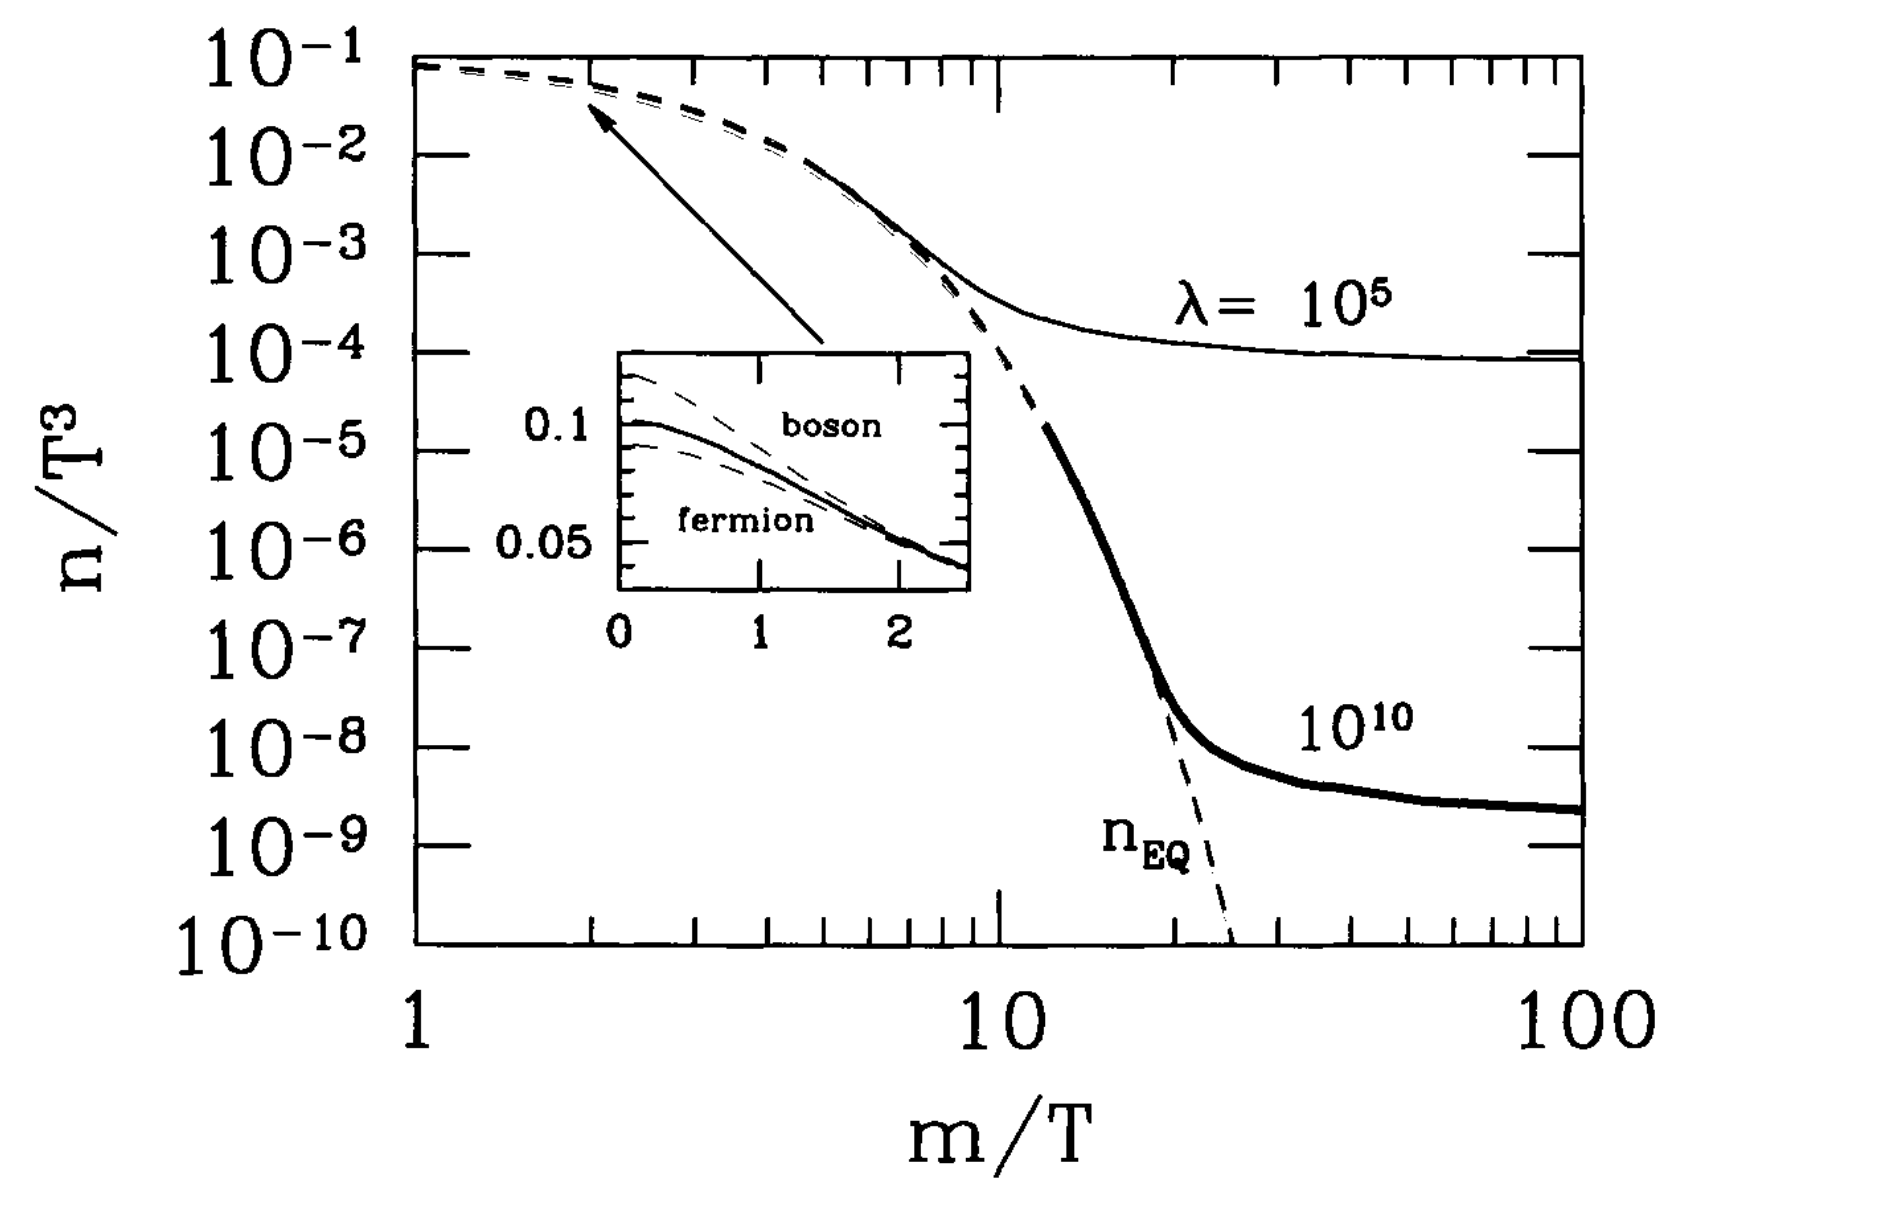
\includegraphics[width=0.8\linewidth]{dmabundance} 
\caption{The abundance of heavy stable particle as the temperature drops beneath its mass. Dashed line is equilibrium abundance. Two different solid curves show heavy particle abundance for two different values of $\lambda$, the ratio of the annihilation rate to the Hubble rate. Inset shows that the difference between quantum statistics and Boltzmann statistics is important only at temperatures larger than the mass. Taken from \cite{Dodelson:2003ft}.}
\label{}
\end{center}
\end{figure}

